\documentclass[10pt]{ctexart}
\usepackage{graphicx, amsmath}
\usepackage{siunitx}
\usepackage[version=4]{mhchem}
\title{微波电子自旋共振和铁磁共振}
\author{张爱强\\指导教师: 王合英}

\date{}
% The following parameters seem to provide a reasonable page setup.

\topmargin 0.0cm
\oddsidemargin 0.2cm
\textwidth 16cm 
\textheight 21cm
\footskip 1.0cm
% set the section title format
\ctexset{
    section/format  += \raggedright
}
% set the abstract format
\newenvironment{sciabstract}{%
\begin{quote} \textbf{摘要: }}
{\end{quote}}
% set the bibliography format
\bibliographystyle{elsarticle-num}


\begin{document}
\maketitle
\begin{sciabstract}
    本实验使用电子自旋共振方法测量顺磁材料中电子的g因子和共振线宽。利用放置在反射式谐振腔中的DPPH样品,测量在正弦磁场中
    电子发生跃迁,从而测量微波自旋共振(ESR)信号,计算出朗德g因子。利用铁磁样品,测量在不同磁场中的吸收强度,测量铁磁样品的弛豫时间。
    \par\textbf{关键词: } 电子自旋共振; g因子;弛豫时间.
\end{sciabstract}
\section{引言}
电子自旋共振谱仪是利用具有未成对电子的物质在静磁场作用下对电磁波的共振吸
收的原理研制的。只有分子中含有未成对电子的物质才可能是 ESR 研究的对象,如自由基、
三重态分子、双基或多基、过渡族金属离子、稀土金属离子以及固体中某些晶格缺陷等。

本实验利用电子自旋共振方法,使用微波器件和示波器测量顺磁材料中电子的g因子和共振线宽,以及铁磁物质的弛豫时间。
\section{实验}
\subsection{实验仪器}
微波器件主要有环形器,单向器,单螺调配器,反射式谐振腔,透射式谐振腔,晶体检波器。

测量ESR实验装置如图~\ref{fig:ESR_instru},测量FMR实验装置如图~\ref{fig:FMR_instru}。
\begin{figure}[htbp]
    \centering
    \begin{minipage}{0.45\textwidth}
        \centering
        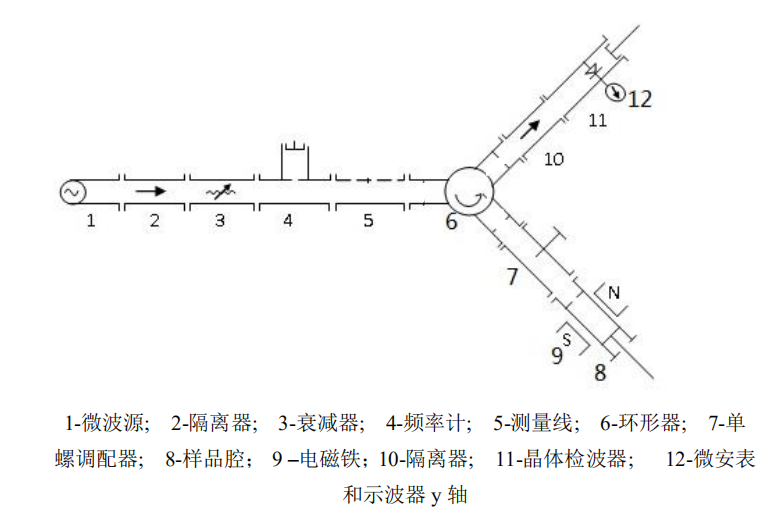
\includegraphics[width=\textwidth]{figure/ESR_instru.png}
        \caption{ESR测量实验装置图}
        \label{fig:ESR_instru}
    \end{minipage}
    \qquad
    \begin{minipage}{0.45\textwidth}
        \centering
        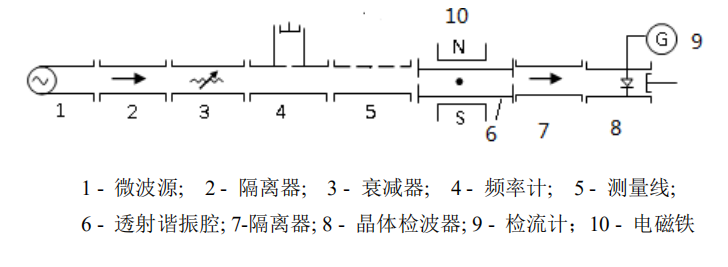
\includegraphics[width=\textwidth]{figure/FMR_instru.png}
        \caption{FMR测量实验装置图}
        \label{fig:FMR_instru}
    \end{minipage}
\end{figure}

\subsection{实验内容}
\subsubsection{ESR}
\begin{enumerate}
    \item 按照图~\ref{fig:ESR_instru}组装微波元件,驻波测量线测量频率
    \item 计算波导波长$\lambda_g$,将DHHP样品置于磁场强度最大处
    \item 调整谐振腔长度使之谐振,调整单螺调配器使谐振腔匹配(可观察到微安表示数为0,其实是基本无反射波)
    \item 加入扫场,找到ESR信号,测量对应的磁场强度
\end{enumerate}
\subsubsection{FMR}
\begin{enumerate}
    \item 按照图~\ref{fig:FMR_instru}组装微波元件,驻波测量线测量频率
\end{enumerate}
\subsubsection{磁场电流标定}
直接使用已标定的结果
\[B=0.1572I+0.0188\]
\section{实验结果及讨论}
\subsection{电子自旋共振}
测量微波频率为
\[f=9.016GHz\]
因此微波波长为$\lambda=c/f=33.3mm$,
实验使用的波导管型号为BJ-100,内腔尺寸为$a=22.86\pm0.07mm$,$b=10.16\pm0.07mm$,
所以波导波长为
\[\lambda_g=\frac{\lambda}{\sqrt{1-(\lambda/2a)^2}}=48.6mm\]
使用的是反射式谐振腔,距离从反射腔入口算起,因为另一端需要调整腔长。谐振腔端面使用的是金属铜片,处于波节处。
样品应放置在
\[d=(2n+1)\lambda_g/2\]
取$n=1$,放置在$d=72.9mm$,调整单螺调配器,使得反射谐振腔匹配。
实际测量过程中,因为微波源并不稳定,所以可能会导致波导中微波频率发生变化。

当发生电子自旋共振时,谐振腔不再匹配,所以会出现反射波,在检波器上会输出电流信号,将信号输入示波器Y轴,扫场信号输入示波器X轴,可以捕获到电子自旋共振
信号。产生电子自旋共振时,检波器输出信号会因为共振减弱,从而出现一个下陷的谷,如图\ref{fig:ESR}。其中两个波谷是因为正弦扫场恰好有两个位置值
对应的频率满足共振频率。调整磁场对应的直流偏置,直到示波器Lisaru图形对应的两个波谷处于两端,恰好相隔半个周期。

\textbf{实际实验过程中只令两个波谷对称,因此在理论上是存在严重问题的,所以会与实际值有一定的偏差。}
\begin{figure}
    \centering
    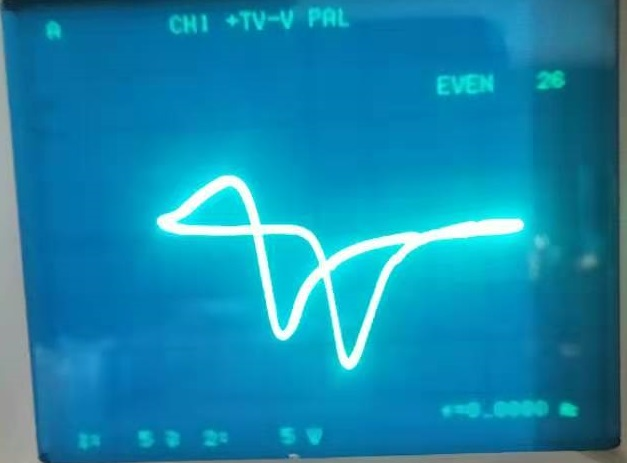
\includegraphics[width=0.7\textwidth]{figure/ESR.jpg}
    \caption{电子自旋共振结果,其中有一个上翘的波峰是由于波导中的频率发生改变导致反射谐振腔不匹配}
    \label{fig:ESR}
\end{figure}
发生电子自旋共振时的电流为$I_{obs}=1.822{\rm A}$,对应的磁场为$B=0.1572I+0.0188=0.3052T$,可以推导出回磁比为
\[\gamma=\frac{\omega}{B}=185.6\times 10^{9}T^{-1}\]
玻尔磁子$\mu_B=e\hbar/2m_e=5.788\times 10^{-11}{\rm MeVT^{-1}}$,普朗克常量$\hbar=6.582\times 10^{-22}{\rm MeVs^{-1}}$,所以算出朗德因子
\[g=\gamma\hbar/\mu_S=2.11\]

\subsection{铁磁共振}
透射式谐振腔腔长为$L$,为了使得谐振腔谐振,需要使得微波频率位于谐振频率附近,此时谐振腔内部的波导波长的整数倍为谐振腔腔长
\[n\lambda_g=L\]
从而可以估计出应处于的谐振频率。

实际调节过程中直接调整微波频率使得微安表示数为0,测量微波频率为
\[f=9.02GHz\]
因此微波波长为$\lambda=c/f=33.3mm$,
所以波导波长为
\[\lambda_g=\frac{\lambda}{\sqrt{1-(\lambda/2a)^2}}=48.6mm\]
发生铁磁共振时的电流为$I_{obs}=1.863A$

实验中测量得到铁磁共振的数据为
\begin{table}
    \begin{tabular}{|c|c|}
        \textbf{I/A} & \textbf{P($\mu A$)}\\
        \hline
        $\infty$  &  32\\
    1.873   & 0\\
    1.876  &  16\\
    1.844  &  16\\
    \end{tabular}
    \centering
    \caption{铁磁P-B数据测量}
    \label{tab:FMR}
\end{table}
所以可以得出P-B曲线的半高宽$\Delta B=0.1572\Delta I=0.1572(1.876-1.844)T=0.005T$那么弛豫时间
\[\tau=2/\gamma/\Delta B=1.08ns\]
\section{结论}
本实验最终给出的\[g=\gamma\hbar/\mu_S=2.11>2\],和理论有差异,考虑到在寻找自旋共振时的电流值存在问题,测量值应该偏小,导致最后对回磁比计算值偏大。
\bibliography{report}
\end{document}